\chapter{背景}
\label{background}

本章では本研究の背景にある既存の知識を整理する。

\section{予言の自己成就現象}
ソーシャルメディア上の根拠のない噂が現実になってしまう現象は、それらが誤った情報であると判明していてもしばらくは続いてしまうことが多い。
メディアではこうした行動は「愚かな行動である」「デマに踊らされている」として説明されることも多いが、それは正しい認識であるとは言えない。
もちろん倫理的な観点からそれらの行動は肯定できるものではないと考えられるが、経済学の観点から考えると合理的であり、むしろそれらの行動をとらないほうが非合理的であるとまでいえるかもしれない。
根拠のない噂が現実となる現象は経済学におけるゲーム理論を用いることで紐解くことができる。
ここから、噂が真実であるか否かに関係なく、噂を現実にしてしまう行動が引き出されることが説明できる。

\section{トイレットペーパー買いだめ問題}
社会情勢が危機的状況になった時、あるいは情報の信憑性に関わらずそうした状況が想定されるとの噂が流れた時、人々がトイレットペーパーをはじめとする日用品の買いだめ行為を行うことが見られる。
新型コロナウイルスの世界的大流行によって,世界各地で外出禁止令が発令されたり、活動の自粛が行われた。
社会的距離の確保(ソーシャルディスタンス)が求められるなか、人々がトイレットペーパーの買いだめ行為に走るという奇妙な現象が起きていたことは記憶に新しい。
きっかけは「中国でトイレットペーパーなどの紙製品が生産されなくなり、日本国内でも大規模な不足が発生する」というソーシャルメディア上での根拠のない情報であった。
この影響で一部ではミネラルウォーターやレトルト食品や米に至るまで品薄となる状況が確認されており、1970年代のオイルショック時の社会的パニック状況を想起させるほどの現象が見られた。
その後上記の情報が誤った情報であると判明しても買いだめ行動は続いた。
これらの行為は「デマに踊らされた大衆の愚かな行為」として説明されることが多い一方で、倫理的観点はさておき、経済学から考えると買いだめ行動はむしろ合理的であるとも捉えることができる。
その論拠について考察する必要がある。

トイレットペーパーをはじめとする日用品の買いだめ行為について、世界中に不安や恐怖が蔓延するなか、コントロールできているという感覚を得ようとしている部分があると顧客行動の研究者であるキット・ヤロウは説明している。
また、不安を感じた際に、それに対処する方法は必ずと言っていいほどコントロールできている感を得ることであるとも説明している。
ウイルス感染拡大の状況を個人がコントロールすることは難しく現実的ではないため、自身がコントロールできる部分に目を向けて行動を起こし準備すること、つまり買いだめをすることであたかも支配権を握っているかのように感じられるということである。


\section{ゲーム理論}
本研究ではゲーム理論を用いてトイレットペーパーの買いだめ問題について取り組む。
ゲーム理論とは数学者ジョン・フォン・ノイマンと経済学者オスカー・モルゲンシュテルンの共著作である「ゲームの理論と経済行動」(1944年)によって誕生した理論である。
この理論を用いることで社会における複数主体が関わる意思決定の問題や行動の相互依存的状況を数学的なモデルを用いて説明することができる。
実際に日常生活やビジネス上の問題、あるいは国家間の問題において自身の行動がどのような結果をもたらすかが、他者のとる行動に強く依存しているケースは多く存在しており、この考え方の適用が可能である。
このように人々の行動が相互依存的関係にある状況を上手く捉えることのできる分析道具がゲーム理論である。
「ゲーム」という言葉が使われていることから分かる通り、問題がどのような構造であるかということやどのようなルールで動いているのか、ということを把握することが重要となるといえる。
構造やルールに応じて戦略をとるという考え方を適用することで効果的に問題の解決に取り組むことができる。

\section{ナッシュ均衡}
ゲーム理論の中で用いられる最も重要な概念の1つにナッシュ均衡がある。
ナッシュ均衡とは、プレーヤー・戦略・利得という構成要素からなるゲーム構造において「相手プレーヤー達の戦略が変わらない時に、自分一人だけが戦略を変えても利得が増えないような戦略の組み合わせ」を示すものである。
言い換えると「自分だけが戦略を変更しても得をしない状態」がナッシュ均衡である。
もし、ゲームの状況がナッシュ均衡でないならば、少なくとも一人は戦略を変化させて得をしようとするプレーヤーが存在することを意味している。
そのため、このような不安定な状況を変化させて、安定的な状況を作り出すことを求める必要がある。
逆にいえば、どのプレーヤーも相手プレーヤー達がナッシュ均衡の戦略を選択しているもとでは最も高い利得を得ているということになる。

\section{囚人のジレンマ}
囚人のジレンマとはゲーム理論におけるゲームの1つである。
お互いが協力する方が協力しないよりも高い利得を得ることが自明な状況であっても、協力しないものが利益を得る状況下では互いに協力しなくなる、というジレンマである。
囚人のジレンマは次のような状況を表している。\\*

共同で罪を犯したと思われる2人の囚人に自白させるため、検事は2人の囚人A・Bに以下の司法取引をもちかける。(2人の囚人は相談できない状況であるとする)\\*

\begin{itemize}
  \item 本来の懲役5年に対して、もし2人とも黙秘をすれば、証拠不十分で減刑して懲役を2年とする
  \item もし片方だけが自白をすれば、当人をその場で釈放して(懲役0年)黙秘した方を懲役10年とする
  \item ただし2人とも自白すれば、本来の判決通り2人とも懲役を5年とする
\end{itemize}

このとき、囚人A・Bはそれぞれ黙秘するべきか、自白するべきかということが問題となる。
この状況下での利得表を以下に示す。\\*

\begin{table}[htbp]
  \centering
  \begin{tabular}{|c|c|c|} \hline
    \diagbox{囚人A}{囚人B} & 黙秘 & 自白 \\ \hline
    黙秘 & (2年,2年) & (10年,0年) \\ \hline
    自白 & (0年,10年) & (5年,5年) \\ \hline
  \end{tabular}
  \caption{囚人のジレンマ:利得表}
  \label{tb:payoff1}
\end{table}

2人の囚人A・Bにとって「互いに自白」して互いに懲役5年の刑を受けるよりは、「互いに黙秘」して互いに2年の刑を受ける方が利得が高い。
しかし、2人の囚人がそれぞれ自分の利益のみを追求する限りにおいては、「互いに黙秘」ではなく「互いに自白」を選択する結果となってしまう。
囚人A・Bそれぞれにとって「互いに黙秘」することが最も利得が高いが、相手がどのように行動するかにかかわらず、2人が共に「自白」することが最適であるといえる。

この概念を買いだめに当てはめると、各消費者はやがて品切れとなり、自身の利得が下がることを避けるために「買いだめをする」という行動をとるようになる。
その結果、集団全体として望ましくない結果をもたらされることを表すことができる。
このように囚人のジレンマを用いて考えることで、買いだめの状況が実現することは説明ができる。
しかしその反面、ナッシュ均衡が1つのみしか存在しない囚人のジレンマでは、普段はなぜ買いだめが起きないのかを説明することができないという問題がある。
そのため、買いだめ問題を考えるにあたり、「囚人のジレンマ」を用いることは最適ではないと考える。

\section{スタグハントゲーム}
スタグハントゲームとは、ゲーム理論における協調ゲームの一種であり、ジャン=ジャック・ルソーの物語「鹿狩りの寓話」に因んで名付けられた概念である。
この概念を用いることで実社会で起きる買いだめの問題を上手く表すことができる。
典型的なスタグハントゲームは次のとおりである。\\*

\begin{itemize}
  \item 2人のハンターは、それぞれrabbitを捕らえて利益1を獲得するか、協力してstagを捕らえて利益2を獲得するかを選択することができる
  \item stagは2人で協力しないと捉えることができないため、1人だけでstagを捕らえようとしても利益は0になってしまう
\end{itemize}

このスタグハントゲームにおける利得表は以下に示したとおりとなる。\\*

\begin{table}[htbp]
  \centering
  \begin{tabular}{|c|c|c|} \hline
    \diagbox{me}{others} & stag & rabbit \\ \hline
    stag & (2,2) & (0,1) \\ \hline
    rabbit & (1,0) & (1,1) \\ \hline
  \end{tabular}
  \caption{スタグハントゲーム:利得表}
  \label{tb:payoff2}
\end{table}

このゲームでは(stag, stag)が2人の利益が共に高い純粋ナッシュ均衡であるが、一方で(rabbit, rabbit)も同じく純粋ナッシュ均衡であるといえる。
stag=1, rabbit=0というように、戦略を数字で定義した場合、利得は2つの数字の最小値に依存する。
すなわち利得は以下のように記述することができる。

\begin{equation}
  \centering
    π_i(s^j_{i},s^k_{-i}) = 1 + 2・min(s^j_{i},s^k_{-i}) - s^j_i
\end{equation}\\*

相手のプレーヤーがstagを選択する確率が高いことが保証されているのであれば、自分もstagを選択するべきである。
しかし相手プレーヤーがrabbitを選択した場合、自身がstagを選択していれば自身の利益は0になってしまう。
つまりスタグハントにおける戦略の不確実性は、プレーヤー間での共通の目的を持ち協力することによる利益2の獲得と、プレーヤーの個人的な目的や相手プレーヤーがrabbitを選択することで利益が0になるリスクを回避することから、自身がrabbitを選択することが対立することによるものである。

囚人のジレンマにおいてナッシュ均衡は「2人とも自白をする」という1つしか存在しないのに対して、スタグハントゲームでは「協力してstagを捕らえる」均衡に加えて「それぞれがrabbitを捕らえる」均衡が存在し、ナッシュ均衡が2つあるという特徴がある。
それにより、この概念を買いだめ問題に当てはめると、買いだめが発生しない「普段の均衡」と「買いだめによる均衡」との2つのナッシュ均衡によって問題を上手く表現することができる。
そのため、囚人のジレンマではなく、スタグハントゲームを用いることにより本研究で扱う買いだめの問題をより正確に表現することができるといえる。
また、スタグハントゲームの概念を買いだめ問題に当てはめると、以下のような利得表が成立すると考えられる。

\begin{table}[htbp]
  \centering
  \begin{tabular}{|c|c|c|} \hline
    \diagbox{自分}{他者} & 普段通りの購買 & 買いだめをする \\ \hline
    普段通りの購買 & (2,2) & (-1,1) \\ \hline
    買いだめをする & (1,-1) & (0,0) \\ \hline
  \end{tabular}
  \caption{買いだめ問題:利得表}
  \label{tb:payoff3}
\end{table}

\section{マルチエージェントシミュレーション}

マルチエージェントシミュレーションとは、人間のように内部状態や行動ルールを持ち、自律的に意思決定を行う「エージェント」と呼ばれるオブジェクトを多数用いて仮想的な社会を作ることで、現実の様々な現象のモデル化を可能にするものである。
一般的にエージェントは、エージェントが自身の行動指針に従って行動する「自律性」、周囲の状況から自身の行動を変化させる「反応性」、周囲と相互依存的な関係にあり、相互作用を生む「社会性」という3つの情報に基づいて処理を進めることができる。
また、マルチエージェントの枠組みでは、これらの特徴を持つエージェントが互いに影響し合い、全体の現象を作り出すことに注目している。
これを用いることで大勢の人間の挙動や動物の群れの様相など、物理的シミュレーションだけでは再現の難しい社会現象や集団の挙動などをシミュレートすることが可能となる。

\section{感染症シミュレーション}
上記のマルチエージェントシミュレーションを用いて、実社会の現象をモデル化して再現した事例として感染症の拡大の様相を表したシミュレーションがある。
複数のエージェントによって形成される社会集団の中で、1エージェントから全体へとウイルスの感染が拡大していく様子を示すことができる。
こうしたシミュレーションを通して、ウイルスが拡散して、感染症が拡大していく構造を認識するとともに、感染拡大の解決となる施策を同シミュレーションで実行することにより、解決に向けた手がかりを得ることが可能となる。

本研究では、感染症シミュレーションを参考に、トイレットペーパーの買いだめのシミュレーションに取り組む。
根拠のない噂が拡散する様相は、根拠のない噂という1つの「ウイルス」が人々のコミュニケーションの中で拡散していくこととして捉えることができる。
また、感染症においてウイルスが拡散して収束する過程で人々は免疫を獲得するが、免疫の獲得は買いだめ問題においては「誤った情報を拡散しないこと」であり、それを通して人々が正しい情報を認識する過程であると示すことができる。
以上を踏まえると、感染症シミュレーションにおけるウイルスの拡散は実社会、特にソーシャルメディア上での根拠のない噂の拡散と同相であると捉えることができると考える。


\if0
\begin{figure}[h]
    \begin{center}
        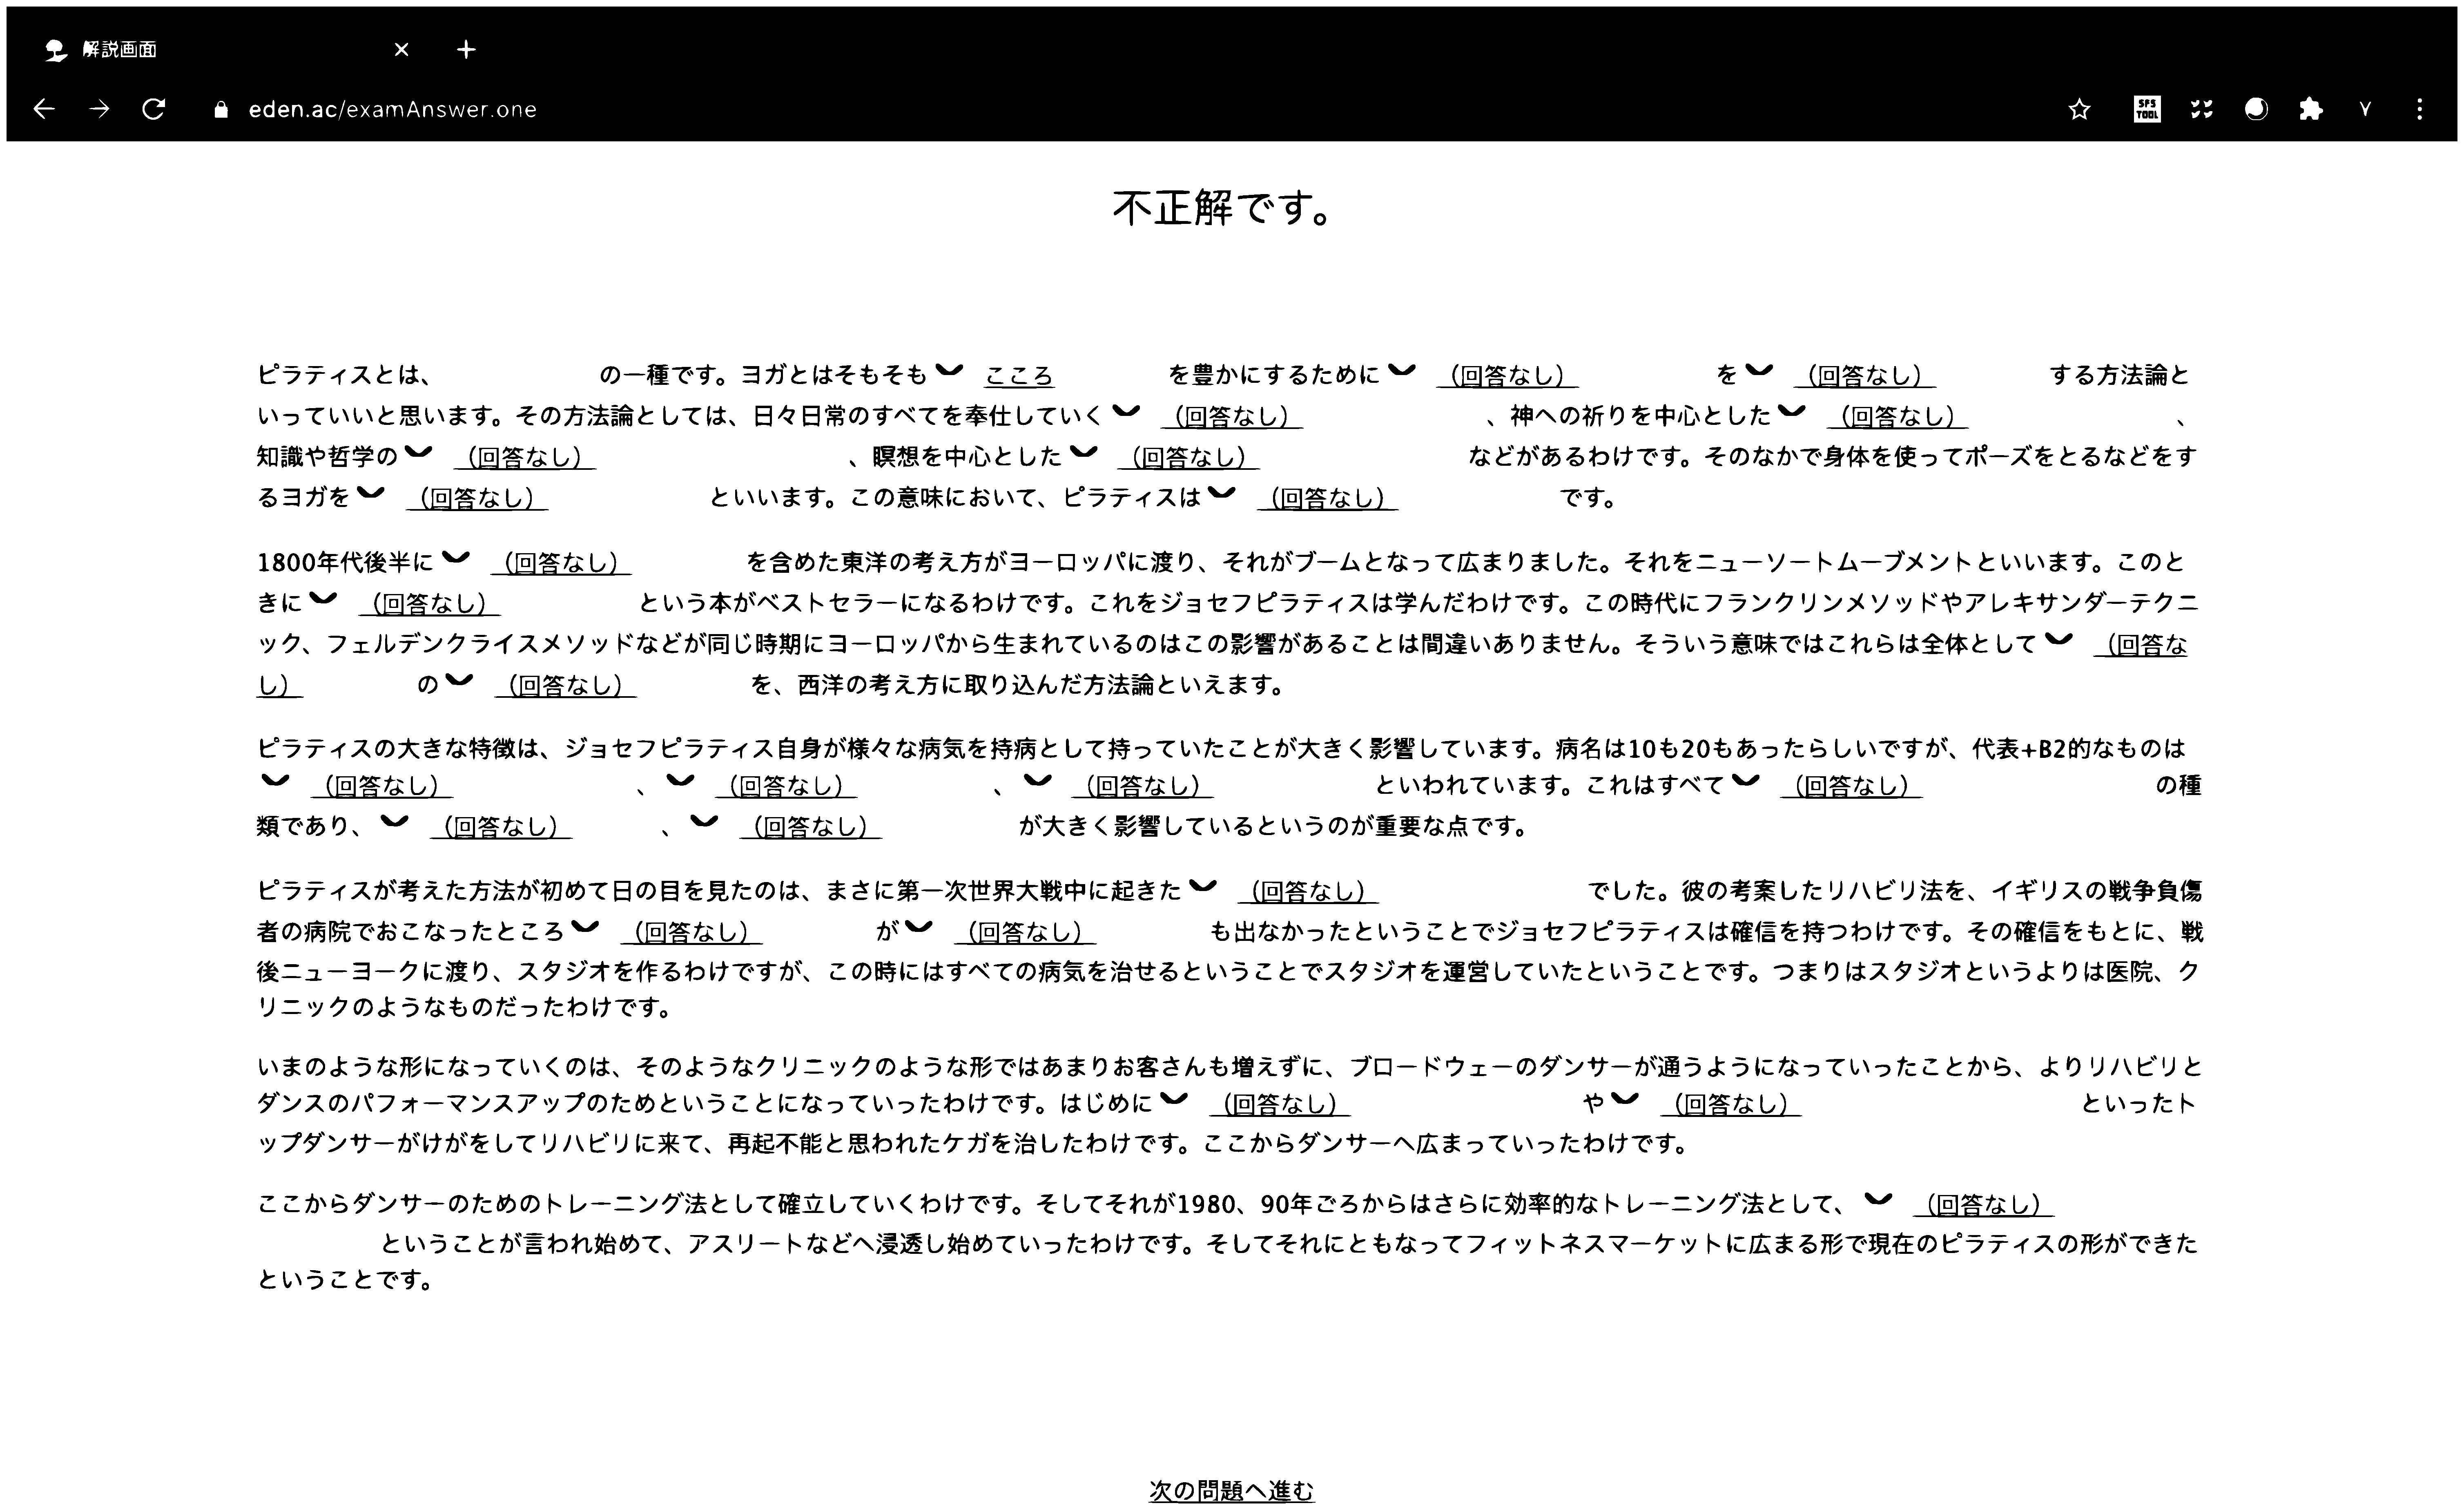
\includegraphics[scale=15cm]{img/hashrate.eps}
        \caption{2017年1月のハッシュレート分布 出典:Blockchain.info\cite{bitcoinhashrate}}
        \label{img:hashrate}
    \end{center}
\end{figure}
\fi

\if0
\begin{figure}[hbtp]
\includegraphics[width=15cm]{img/auzrk-ytelz.eps}
	\caption{活性化関数の歴史}
	\label{history_af}
\end{figure}
\fi